\documentclass[12pt]{article}
\usepackage[a4paper,margin=1.6cm]{geometry}
\usepackage{amsmath,amssymb}
\usepackage{tikz}
\usetikzlibrary{arrows.meta,positioning,decorations.pathmorphing}
\usepackage{array}
\usepackage{helvet}
\renewcommand{\familydefault}{\sfdefault}
\pagestyle{empty}

\begin{document}
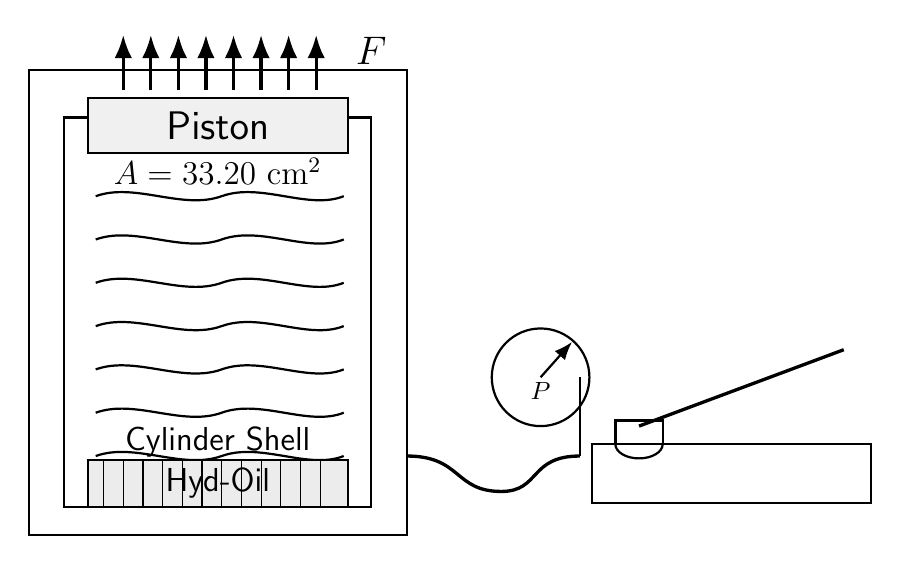
\begin{tikzpicture}[x=1cm,y=1cm,>=Latex,font=\sffamily]
  % Hydraulic cylinder
  \draw[thick] (0,0) rectangle (4.8,5.9);
  \draw[thick] (0.45,0.35) rectangle (4.35,5.3);
  \draw[thick,fill=gray!12] (0.75,4.85) rectangle (4.05,5.55);
  \node at (2.4,5.2) {\Large Piston};
  \draw[thick] (0.75,4.85) -- (4.05,4.85);
  % spring / fluid lines
  \foreach \y in {1.0,1.55,2.1,2.65,3.2,3.75,4.3}
    \draw[thick] (0.85,\y) .. controls (1.35,\y+0.18) and
      (1.95,\y-0.18) .. (2.45,\y)
      .. controls (2.95,\y+0.18) and (3.55,\y-0.18) .. (4.0,\y);
  \draw[thick,fill=gray!15] (0.75,0.35) rectangle (4.05,0.95);
  \foreach \x in {0.95,1.2,1.45,1.7,1.95,2.2,2.45,2.7,2.95,3.2,3.45,3.7}
    \draw (\x,0.35) -- (\x,0.95);
  \node at (2.4,0.65) {\large Hyd-Oil};
  \node[align=center] at (2.4,1.18) {\large Cylinder Shell};
  \node[align=center] at (2.4,4.62) {\large $A=33.20\ \mathrm{cm^2}$};
  % upward force arrows
  \foreach \x in {1.2,1.55,1.9,2.25,2.6,2.95,3.3,3.65}
    \draw[very thick,->] (\x,5.65) -- (\x,6.35);
  \node at (4.35,6.15) {\Large $F$};
  % hose
  \draw[very thick] (4.8,1.0) .. controls (5.5,1.0) and (5.4,0.55) ..
    (6.0,0.55) .. controls (6.5,0.55) and (6.35,1.0) .. (7.0,1.0);
  % gauge
  \draw[thick] (7.0,1.0) -- (7.0,2.0);
  \draw[thick] (6.5,2.0) circle (0.62);
  \draw[thick,->] (6.5,2.0) -- (6.9,2.45);
  \node at (6.5,1.82) {\small $P$};
  % pump and lever
  \draw[thick] (7.15,0.4) rectangle (10.7,1.15);
  \draw[thick] (7.45,1.15) rectangle (8.05,1.45);
  \draw[very thick] (7.75,1.38) -- (10.35,2.35);
  \draw[thick] (7.45,1.15) arc (180:360:0.3 and 0.18);
  \node[below=0.15cm] at (8.95,0.4) {};
\end{tikzpicture}

\vspace{0.4cm}
\noindent\hrulefill
\vspace{0.55cm}

\begin{align*}
F &= G = m g
   = (5000\ \mathrm{kg})(9.8\ \mathrm{N/kg})
   = 49\,000\ \mathrm{N},\\[0.4em]
A &= 33.20\ \mathrm{cm^2}
   = 33.20\times10^{-4}\ \mathrm{m^2}
   = 3.320\times10^{-3}\ \mathrm{m^2},\\[0.4em]
P &= \frac{F}{A}
   = \frac{(5000\ \mathrm{kg})(9.8\ \mathrm{N/kg})}
          {33.20\times10^{-4}\ \mathrm{m^2}}\\[0.25em]
  &= 1.4759\times10^{7}\ \mathrm{Pa}
   \approx \boxed{14.76\ \mathrm{MPa}}.
\end{align*}

\vfill
\noindent\rule{\textwidth}{0.5pt}\\[-0.2em]
\small
\makebox[2.2cm][l]{Checked by}\hfill
\makebox[2.4cm][l]{Approved}\hfill
\makebox[2.0cm][r]{Date}
\end{document}
